\newcommand{\cccnormspacing}{\baselineskip=12pt}
\newcommand{\cccnormspacingcenter}{\centering\arraybackslash\cccnormspacing}


\section{Analisis Kebutuhan Pengguna}

Setelah mengidentifikasi konteks penggunaan dari aplikasi Digital Wellbeing, dilakukan analisis terhadap kebutuhan pengguna. Kebutuhan-kebutuhan ini 

\subsection{Skenario Pengguna}
\subsection{Analisis Fitur}
\subsection{Analisis Prinsip Desain}
\subsection{Analisis Usability dan User Experience Goal}

% Proses perancangan solusi mengacu kepada metode \textit{User-Centered Design} sesuai dengan standar ISO 9241-210, di mana pada tahap perancangan desain interaksi untuk memenuhi kebutuhan pengguna akan disertai dengan prototipe aplikasi. Gambar \ref{fig:diagram_alur_kerja} menjelaskan tentang alur kerja penelitian yang dilakukan.

% \begin{figure}[h]
%   \centering
%   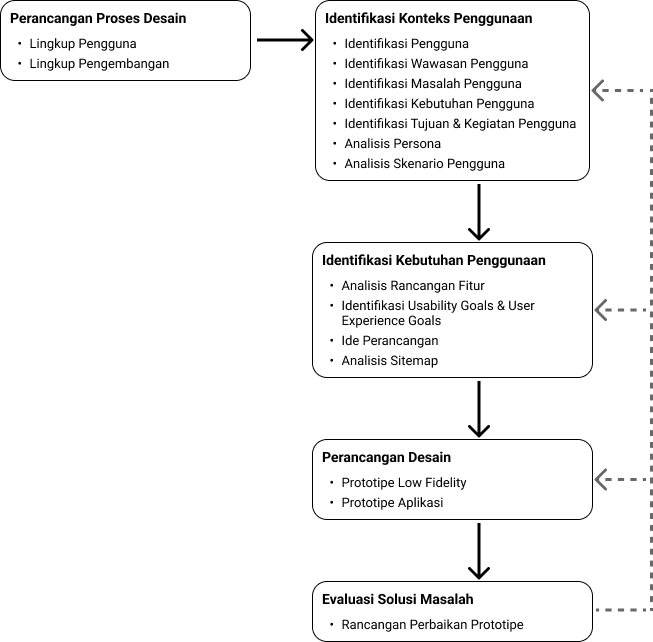
\includegraphics[width=0.8\textwidth]{chapter-3-alur-penelitian.png}
%   \caption{Alur Kerja Penelitian}
%   \label{fig:diagram_alur_kerja}
% \end{figure}

% \subsection{Perancangan Proses Desain}
% Ruang lingkup yang ditentukan pada penelitian ini adalah sebagai berikut

% \begin{enumerate}
%   \item Lingkup Pengguna
%   \subitem Target pengguna dari penelitian ini adalah masyarakat Indonesia yang pernah menggunakan atau memiliki ketertarikan terhadap aplikasi pencegah distraksi. Rentang usia dari target pengguna tidak dibatasi, namun difokuskan kepada golongan \textit{millenials} dengan rentang usia 18-30 tahun.
%   \item Lingkup Pengembangan
%   \subitem Desain interaksi aplikasi pencegah distraksi yang dibuat memiliki bentuk \textit{mobile interface} dengan mewujudkan sebuah prototipe aplikasi dalam \textit{platform Android}. Aplikasi Digital Wellbeing milik Google ditetapkan menjadi garis dasar pengembangan prototipe aplikasi tersebut.
% \end{enumerate}


% \subsection{Identifikasi Konteks Penggunaan}

% Pada tahap ini dilakukan analisis hasil riset penggunaanalisis terhadap hasil riset yang


% \subsection{Identifikasi Kebutuhan Pengguna}


% \subsection{Perancangan Desain}


% \subsection{Evaluasi Solusi Masalah}



% % Ketiga solusi yang telah diuraikan pada subbab \ref{sec:analisis_solusi} akan diimplementasikan dalam prototipe aplikasi, beserta fitur-fitur lain pada Digital Wellbeing yang akan mendukung solusi tersebut. Prototipe aplikasi ini akan diimpementasikan pada \textit{platform} Android. Secara garis besar, proses perancangan prototipe aplikasi akan menggunakan pendekatan \textit{user-centered design} (UCD).

% Seperti yang telah disebutkan pada subbab \ref{sec:metodologi}, metodologi yang digunakan dalam pengerjaan Tugas Akhir ini akan menggunakan pendekatan UCD. Dengan maksud mengikuti prosesnya, maka langkah selanjutnya yang akan dilakukan adalah mengumpulkan data. Pengumpulan data akan dilakukan dengan menyebarkan form secara online serta melakukan wawancara dengan responden yang bersedia untuk bekerja sama lebih lanjut. Proses ini akan dilaksanakan pada periode pengerjaan Tugas Akhir 2. Pengumpulan data ini bertujuan untuk melakukan validasi terhadap permasalahan yang sudah dianalisis, dan juga tidak menutup kemungkinan untuk menemukan permasalahan desain interaksi lain dari masukan pengguna.

% Setelah melakukan pengumpulan data, akan dilakukan analisis terhadap masukan yang didapat untuk mejadi kebutuhan perangkat lunak. Hasil analisis juga akan memvalidasi analisis masalah dan solusi yang didapat dari observasi penulis pada subbab \ref{sec:analisis_masalah} dan \ref{sec:analisis_solusi}.

% Kebutuhan perangkat lunak yang telah disusun akan diimplementasi dalam bentuk prototipe \textit{low-fidelity} terlebih dahulu. Setelah dilakukan evaluasi, maka implementasi akan dilanjutkan dalam bentuk prototipe \textit{high-fidelity}. Setelah menjalani evaluasi, maka perancangan prototipe aplikasi akan dikerjakan. Prototipe aplikasi diharapkan akan menghasilkan data dengan kualitas yang lebih tinggi pada saat evaluasi dibandingkan saat menggunakan prototipe \textit{low-fidelity} atau \textit{high-fidelity}. Hasil evaluasi juga akan menentukan apakah aplikasi akan menjalani proses iterasi atau diimplementasi lebih lanjut.

% \blindtext